\documentclass[Royal,times,sageh]{sagej}

\usepackage{moreverb,url,natbib, multirow, tabularx}
\usepackage[colorlinks,bookmarksopen,bookmarksnumbered,citecolor=red,urlcolor=red]{hyperref}



% tightlist command for lists without linebreak
\providecommand{\tightlist}{%
  \setlength{\itemsep}{0pt}\setlength{\parskip}{0pt}}



\usepackage{booktabs}
\usepackage{longtable}
\usepackage{array}
\usepackage{multirow}
\usepackage{wrapfig}
\usepackage{float}
\usepackage{colortbl}
\usepackage{pdflscape}
\usepackage{tabu}
\usepackage{threeparttable}
\usepackage{threeparttablex}
\usepackage[normalem]{ulem}
\usepackage{makecell}
\usepackage{xcolor}


\begin{document}


\setcitestyle{aysep={,}}

\title{ActiveCA: Time Use Data from the General Social Survey of Canada
to Study Active Travel}

\runninghead{}

\author{Anon1\affilnum{}, Anon2\affilnum{}, Anon3\affilnum{}}

\affiliation{\affilnum{}{}}



\begin{abstract}
This paper describes \{ActiveCA\}, and open data product with Canadian
time use data. \{ActiveCA\} is an \texttt{R} data package that contains
analysis-ready data related to active travel spanning almost 40 years,
extracted from cycles 2 (1986), 7 (1992), 12 (1998), 19 (2005), 24
(2010), and 29 (2015) of Canada's General Social Survey. Active travel
is characterized by mode, with walking being part of every cycle and
bicycling starting in 1992. The attributes of active trips are the types
of locations of origins and destinations, the duration of trips, and
episode weights for expanding the trips to population-wide estimates.
Based on the year of the survey, a variety of locations are coded. In
earlier cycles, these include home, work or school, and other's home,
whereas in later cycles these are augmented with locations such as
grocery stores, restaurants, outdoor destinations, and others. The
geographical resolution includes the province and whether the episode
was in an urban or rural setting.
\end{abstract}

\keywords{Active; mobility; walking; cycling; travel time; time-use;
General Social Survey}

\maketitle

\section{Introduction}\label{introduction}

The objective of this paper is to introduce \{ActiveCA\}, an open data
product with time use data from Canada's General Social Surveys. Open
data products (ODPs) are the outcome of a process that transforms raw
data (open or not) into analysis-ready data, following a transparent
process in which all stages of development follow open principles
\citep{arribas-bel2021}. ODPs, while still open, differ from general
open data in their degree of ease of access, their heightened usability,
and potentially the value they add to the raw data.

\{ActiveCA\} provides analysis-ready data concerning active travel in
Canada spanning a period of almost 40 years. The source of these data is
Canada's program of General Social Surveys (GSSs). This program is
designed to provide cross-sectional data on topics of interest to
improve the well-being of Canadians. As part of this program, every five
to seven years the survey is done on the topic of time use. Concretely,
\{ActiveCA\} covers Cycles 2 (1986), 7 (1992), 12 (1998), 19 (2005), 24
(2010), and 29 (2015) of the GSS. Time use data in these surveys is
coded using a very fine grain, from time spent in chores, leisure, and
sleeping, to time spent working or at school. These surveys have proved
valuable in investigations of mobility and quality of life
\citep{spinneyTransport2009}, the relationship between active travel and
transit use \citep{lachapelleLonger2016}, and travel behavior and time
poverty \citep{kimFacing2024}, to name but a few examples.

For \{ActiveCA\} and using GSS Public Use Microdata Files (PUMFs), we
extracted all data needed to characterize active travel in Canada,
namely, episodes where the activity was identified as moving between an
origin and a destination, either by walking or cycling. Although
Statistics Canada offers Public Use Microdata Files and documentation
for the GSS program \citep[see][]{statisticscanada2024}, accessing these
files, and preparing them for analysis is not a straightforward matter,
given their size and complexity. The process of extracting information
of interest from the source files is time-consuming, tedious, and
challenging and/or prone to error due to the expertise required to work
with these files. To create \{ActiveCA\} we collected, cleaned, and
processed the cycles of the GSS surveys concerning time use to make them
ready for analysis.

\{ActiveCA\} is distributed as an \texttt{R} package with a number of
data objects and their documentation. \texttt{R} packages contain code,
data, and documentation in a standardized format that can be installed
by \texttt{R} users via a software repository, such as CRAN
(Comprehensive R Archive Network) or GitHub, which makes them an adroit
medium to distribute analysis-ready data.

Given the level of interest in active travel
\citep[e.g.,][]{mccurdySupport2023}, reducing the barriers to using data
contained in rich, but difficult to access and use surveys, such as
Canada's GSSs, is a worthy endeavour that can only improve data-driven
decisions in transportation, urban, and health policy.

The rest of this paper discusses the sources of data, and the process
implemented to retrieve and package them. Then, we explain how to use
the package and show some selected examples of analysis to whet the
imagination of potential users. This ODP provides not only data that are
easy to use, but also all the code and documentation that make this a
reproducible research project. In summary, \{ActiveCA\} aims to
implement and inspire the best principles of open spatial sciences
\citep{paez_open_2021, brunsdon_opening_2021}.

\section{General Social Survey (GSS)
collection}\label{general-social-survey-gss-collection}

Statistics Canada \citeyearpar{statisticscanada2024} conducts GSS
surveys to obtain data on social trends to track changes in Canadians'
living conditions and well-being over time. The series of survey on time
use are used to understand how Canadian residents spend and manage their
time, and what factors contribute to their happiness and stress. The GSS
program was created in 1985, and is serialized to provide a collection
of annual, representative cross-sectional surveys.

The topics of the survey cycle every few years to cover topics that
include family, health, social identity, and every five to seven years
time use. The first Canadian time use survey done as part of the GSS
program was conducted in 1986, and the most recent was completed in
2015. These Time Use Surveys \citep{statisticscanada2022} collect data
on respondents' participation and time spent on a wide range of everyday
activities using a 24-hour retrospective diary, with information on the
location of these activities (e.g.~at home, at work, etc.) and, for
non-personal activities, the people who were present with the respondent
at the time of the activity. In addition, time-use surveys also cover
topics related to leisure time, work-life balance, health, commuting,
culture and sports, and many others.

The Public Use Microdata are released by Statistics Canada in two files:
a \emph{Main File} and an \emph{Episode File}. The files are linked by
keys that identify households, individuals, and episodes (i.e.,
activities) conducted by individuals. We discuss these files in more
detail in the following section.

\subsection{The Main File}\label{the-main-file}

The main file of the time use survey compiles a large array of
aggregated data, summarizing the answers to the questionnaire that
describe households and individuals, as well as derived variables that
summarize the respondents' use of time use across different activities,
locations, and social interactions. This file documents the time and
duration that respondents allocate to each activity and location. The
Main File provides a overview of daily routines and social dynamics, not
focusing on individual activity episodes. Additionally, this file
categorizes activities into bigger groups and subcategories,
facilitating the data's analytical utility with additional metrics such
as total transit time, time spent with household members, and counts of
activities and episodes.

The table \ref{tab:main-2015-unprocessed} shows the first ten lines and
the first 6 variables of the GSS PUMF 2015 main file (Cycle 29). Each
line of the table refers to a respondent in a survey and the columns
refer respectively to the record identification (\texttt{PUMFID}), the
person's weight (\texttt{WGHT\_PER}), the month the survey data was
collected (\texttt{SURVMNTH}), the respondent's age group
(\texttt{AGEGR10}), the respondent's sex (\texttt{SEX}), and the
respondent's marital status (\texttt{MARSTAT}). In total, the main file
of the 2015 GSS surveys has 17,390 respondents corresponding to
\ensuremath{2.9766399\times 10^{7}} people and 848 variables. For the
discrete variables, Statistic Canada has created codes for the possible
values and each value has its own label. For example, for the variable
\texttt{SURVMNTH}, the value \texttt{1} means \texttt{January\ 2016},
while 2 means \texttt{February\ 2016}, 3 is \texttt{March\ 2016} and so
on. As you can see from the example in Table
\ref{tab:main-2015-unprocessed}, the variables are not labeled. In
addition, the format of the tables (comma separated) does not allow you
to specify the type of each variable (whether it is continuous or
discrete, for example), which can cause confusion for an analyst with
relatively little experience in handling PUMFs.

\begingroup\fontsize{8}{10}\selectfont

\begin{ThreePartTable}
\begin{TableNotes}
\item \textit{Note: } 
\item Legend: `PUMFID`: record identification. `WGHT\_PER`:  person weight. `SURVMNTH`: survey month of data collection. `AGEGR10`: age group of the respondent. `SEX`: sex of the respondent. `MARSTAT`: marital status of the respondent.
\end{TableNotes}
\begin{longtable}[t]{cccccc}
\caption{\label{tab:gss-main-file-2015}\label{tab:main-2015-unprocessed}Visualization of the first ten lines and first six columns of the main file of the 2015 GSS.}\\
\toprule
PUMFID & WGHT\_PER & SURVMNTH & AGEGR10 & SEX & MARSTAT\\
\midrule
10000 & 616.6740 & 7 & 5 & 1 & 5\\
10001 & 8516.6140 & 7 & 5 & 1 & 1\\
10002 & 371.7520 & 1 & 4 & 2 & 1\\
10003 & 1019.3135 & 3 & 6 & 2 & 5\\
10004 & 1916.0708 & 9 & 2 & 1 & 6\\
\addlinespace
10005 & 1952.2015 & 4 & 1 & 1 & 6\\
10006 & 5761.5528 & 8 & 1 & 1 & 6\\
10007 & 466.0426 & 6 & 5 & 2 & 3\\
10008 & 2479.2991 & 2 & 2 & 2 & 1\\
10009 & 1436.1641 & 8 & 6 & 1 & 3\\
\bottomrule
\insertTableNotes
\end{longtable}
\end{ThreePartTable}
\endgroup{}

\subsection{The Episode File}\label{the-episode-file}

The episode is a much bigger file that records detailed data for each
activity episode reported by respondents. Each episode represents a
single activity and its duration, and the sum of all episodes throughout
the day adds up to 24 hours. Each entry in this file includes the start
and end times of the activity, the duration, location, and accompanying
social context, informing when and where activities occurred and with
whom. The focus of the Episode File is not on the characteristics of the
respondents, but on the characteristics of the activities, and the data
are structured around the numerous activity instances that compose a day
of the respondent. Although respondent-specific characteristics are not
included within the episode file, it is possible to link the main file
and the episode file by using a key present in both the Main and Episode
Files.

Similarly to Table \ref{tab:main-2015-unprocessed} that displayed an
example of the main file structure, Table \ref{tab:ep-2015-unprocessed}
shows the first seven episodes for the record identification number
\texttt{10041} and some variables of the GSS PUMF 2015 episode file
(Cycle 29). Each line of the table refers to an episode of the
especified record identification (\texttt{PUMFID\ =\ 10041}), the
episode's weight (\texttt{WGHT\_EPI}), the episode number
(\texttt{EPINO}), the activity code (\texttt{TUI\_01}), the episode's
duration (\texttt{DURATION}) and the episode's location
(\texttt{LOCATION}). In total, the episode file of the 2015 GSS surveys
has 274,108 records corresponding to \ensuremath{4.6183762\times 10^{8}}
episodes and 527 variables that detail the episodes. As similar to the
main file, Statistic Canada has created codes for the possible values of
the discrete variables with each value has its own label. Considering
the case displayed in Table \ref{tab:ep-2015-unprocessed}, this person
started the diary description while sleeping at home
(\texttt{TUI\_01\ =\ 1} and \texttt{LOCATION\ =\ 300}) for 210 minutes,
then engaged in personal hygiene for 40 minutes
(\texttt{TUI\_01\ =\ 2}), then spent 15 minutes getting personal care
(which can be getting ready for school, supervising homework, reading,
playing, reprimanding, educational, or emotional help, sinalized by the
\texttt{TUI\_01\ =\ 27}). After this, this person had an activity travel
episode, walking for 15 minutes (\texttt{TUI\_01\ =\ 7} and
\texttt{LOCATION\ =\ 315}) in which the origin and destination was their
own house. Cases like this, where the trip starts and finishes at home
refers to recreational and leisure trips. After that, the person spent 3
hours looking for a job (\texttt{TUI\_01\ =\ 9}), had break for a lunch
of 15 minutes duration (\texttt{TUI\_01\ =\ 6}) and cleaned the house
(\texttt{TUI\_01\ =\ 18}) for two hours. Table
\ref{tab:ep-2015-unprocessed} shows only six variables from the 527
possible cases. As you can see, since that data set is not labeled,
figuring out the codes for every variable can be time consuming and
difficult.

\begingroup\fontsize{8}{10}\selectfont

\begin{ThreePartTable}
\begin{TableNotes}
\item \textit{Note: } 
\item Legend: `PUMFID`: record identification. `EPINO`: episode number. WGHT\_EPI: episode's weight. TUI\_01: activity code. DURATION: episode's duration. LOCATION: episode's location.
\end{TableNotes}
\begin{longtable}[t]{cccccc}
\caption{\label{tab:gss-epi-file-2015}\label{tab:main-2015-unprocessed}Visualization of the seven first episodes of the record number `10041`.}\\
\toprule
PUMFID & EPINO & WGHT\_EPI & TUI\_01 & DURATION & LOCATION\\
\midrule
10041 & 1 & 1353.818 & 1 & 210 & 300\\
10041 & 2 & 1353.818 & 2 & 40 & 300\\
10041 & 3 & 1353.818 & 27 & 15 & 300\\
10041 & 4 & 1353.818 & 7 & 15 & 315\\
10041 & 5 & 1353.818 & 9 & 180 & 300\\
\addlinespace
10041 & 6 & 1353.818 & 6 & 15 & 300\\
10041 & 7 & 1353.818 & 18 & 120 & 300\\
\bottomrule
\insertTableNotes
\end{longtable}
\end{ThreePartTable}
\endgroup{}

\section{Data extraction}\label{data-extraction}

For each selected cycle of the GSS surveys, we reviewed the episode
files to identify episodes of movement that involved walking or cycling.
This allowed us to select the activities immediately before and after
the movement episode. After that, we labeled the code variables with
their appropriate descriptions, identifying each origin and destination,
mode of travel, as well the province and urban classification of the
episode.

\section{How to use \{ActiveCA\}}\label{how-to-use-activeca}

\subsection{Descriptive statistics}\label{descriptive-statistics}

Considering GSS Cycles analyzed, we identified 21748 episodes that
recorded active travel episodes, with trip duration ranging from 0 to
900 minutes, to twelve different destinations. \texttt{ActiveCA}
includes all these episodes ready for analysis. Table \ref{tab:table-01}
presents descriptive statistics on walking and cycling trips between
1986 and 2015, including metrics such as the count of recorded trips
(count), and measures of trip duration in minutes: maximum (max), mean,
median, and minimum (min). The 1986 survey did not include bicycle
trips.

\begingroup\fontsize{10}{12}\selectfont

\begin{longtable}[t]{>{}llcccccc}
\caption{\label{tab:table-01}\label{tab:table-01}Descriptive statistics for episodes with active transport records}\\
\toprule
\multicolumn{2}{c}{ } & \multicolumn{6}{c}{Year} \\
\cmidrule(l{3pt}r{3pt}){3-8}
Mode & Statistic & 1986 & 1992 & 1998 & 2005 & 2010 & 2015\\
\midrule
 & Count & 4347 & 1500 & 1670 & 5533 & 4379 & 3251\\
\nopagebreak
 & Maximum & 660 & 300 & 255 & 515 & 480 & 900\\
\nopagebreak
 & Mean & 21 & 19 & 11 & 12 & 12 & 17\\
\nopagebreak
 & Median & 10 & 10 & 5 & 10 & 8 & 10\\
\nopagebreak
 & Minimum & 1 & 1 & 1 & 0 & 0 & 5\\
\nopagebreak
\multirow[t]{-6}{*}{\raggedright\arraybackslash \textbf{Walking}} & Standard deviation & 31 & 25 & 17 & 16 & 17 & 27\\
\cmidrule{1-8}\pagebreak[0]
 & Count &  & 135 & 119 & 333 & 236 & 245\\
\nopagebreak
 & Maximum &  & 240 & 90 & 180 & 153 & 120\\
\nopagebreak
 & Mean &  & 31 & 21 & 19 & 21 & 24\\
\nopagebreak
 & Median &  & 20 & 15 & 15 & 15 & 15\\
\nopagebreak
 & Minimum &  & 5 & 2 & 1 & 1 & 5\\
\nopagebreak
\multirow[t]{-6}{*}{\raggedright\arraybackslash \textbf{Cycling}} & Standard deviation &  & 36 & 18 & 18 & 23 & 20\\
\bottomrule
\end{longtable}
\endgroup{}

Table \ref{tab:table-01} shows that the median values for walking trips
range between 5 and 10 minutes, while cycling trips have a consistent
median of 15 minutes since 1998. The table also highlights very high
maximum values, particularly for walking trips, with recorded episodes
exceeding 4 hours in all cases.

Table \ref{tab:table-02} and \ref{tab:table-03} provide descriptive
statistics for the two modes of transportation, split by destination
categories, from 1986 to 1998 and from 2005 to 2015, respectively. In
Table \ref{tab:table-02}, one can observed that in 1986 and 1992,
walking trips destined for \texttt{home} had the highest medians.
However, by 1998, the highest medians shifted to trips to
\texttt{work\ or\ school}, a transition that also occurred for cycling
trips between 1992 and 1998. Table \ref{tab:table-03} indicates that the
median duration for trips to \texttt{home} and \texttt{work\ or\ school}
remained at 10 minutes.

\begingroup\fontsize{6}{8}\selectfont

\begin{ThreePartTable}
\begin{TableNotes}
\item \textit{Note: } 
\item * The symbols used in this table represent the following: 'Min' denotes the minimum time to reach the destination; 'Max' denotes the maximum time to reach the destination; '(\%)' indicates a percentage of the total time to reach the destination; 'Med' refers to the median time to reach the destination
\end{TableNotes}
\begin{longtable}[t]{ccccc>{}c|ccc>{}c|cccc}
\caption{\label{tab:table-02}\label{tab:table-02}Comparison of travel statistics by mode and destination: 1986, 1992, 1998}\\
\toprule
\multicolumn{2}{c}{ } & \multicolumn{4}{c}{1986} & \multicolumn{4}{c}{1992} & \multicolumn{4}{c}{1998} \\
\cmidrule(l{3pt}r{3pt}){3-6} \cmidrule(l{3pt}r{3pt}){7-10} \cmidrule(l{3pt}r{3pt}){11-14}
\multicolumn{1}{c}{\textbf{Destination}} & \multicolumn{1}{c}{\textbf{Mode*}} & \multicolumn{1}{c}{\textbf{Min*}} & \multicolumn{1}{c}{\textbf{Med*}} & \multicolumn{1}{c}{\textbf{Max*}} & \multicolumn{1}{c}{\textbf{(\%)*}} & \multicolumn{1}{c}{\textbf{Min}} & \multicolumn{1}{c}{\textbf{Med}} & \multicolumn{1}{c}{\textbf{Max}} & \multicolumn{1}{c}{\textbf{(\%)}} & \multicolumn{1}{c}{\textbf{Min}} & \multicolumn{1}{c}{\textbf{Med}} & \multicolumn{1}{c}{\textbf{Max}} & \multicolumn{1}{c}{\textbf{(\%)}}\\
\midrule
 & Home &  &  &  &  & 5 & 20 & 240 & 55.6 & 2 & 15.0 & 90 & 52.9\\
\nopagebreak
 & Other's home &  &  &  &  & 5 & 10 & 145 & 18.5 & 2 & 10.0 & 80 & 17.6\\
\nopagebreak
\multirow[t]{-3}{*}{\centering\arraybackslash Cycling} & Work or school &  &  &  &  & 5 & 15 & 45 & 25.9 & 5 & 20.0 & 75 & 29.4\\
\cmidrule{1-14}\pagebreak[0]
 & Home & 1 & 15 & 330 & 46.4 & 1 & 10 & 300 & 59.5 & 1 & 5.0 & 255 & 51.6\\
\nopagebreak
 & Other's home & 1 & 10 & 660 & 42.3 & 1 & 5 & 135 & 21.3 & 1 & 5.0 & 120 & 28.1\\
\nopagebreak
\multirow[t]{-3}{*}{\centering\arraybackslash Walking} & Work or school & 1 & 10 & 450 & 11.3 & 2 & 10 & 60 & 19.2 & 1 & 6.5 & 75 & 20.4\\
\bottomrule
\insertTableNotes
\end{longtable}
\end{ThreePartTable}
\endgroup{}

\begingroup\fontsize{6}{8}\selectfont

\begin{ThreePartTable}
\begin{TableNotes}
\item \textit{Note: } 
\item * The symbols used in this table represent the following: 'Min' denotes the minimum time to reach the destination; 'Max' denotes the maximum time to reach the destination; '(\%)' indicates a percentage of the total time to reach the destination; 'Med' refers to the median time to reach the destination
\end{TableNotes}
\begin{longtable}[t]{ccccc>{}c|ccc>{}c|cccc}
\caption{\label{tab:table-03}\label{tab:table-03}Comparison of travel statistics by mode and destination: 2005, 2010, 2015}\\
\toprule
\multicolumn{2}{c}{ } & \multicolumn{4}{c}{2005} & \multicolumn{4}{c}{2010} & \multicolumn{4}{c}{2015} \\
\cmidrule(l{3pt}r{3pt}){3-6} \cmidrule(l{3pt}r{3pt}){7-10} \cmidrule(l{3pt}r{3pt}){11-14}
\multicolumn{1}{c}{\textbf{Destination}} & \multicolumn{1}{c}{\textbf{Mode}} & \multicolumn{1}{c}{\textbf{Min*}} & \multicolumn{1}{c}{\textbf{Med*}} & \multicolumn{1}{c}{\textbf{Max*}} & \multicolumn{1}{c}{\textbf{(\%)*}} & \multicolumn{1}{c}{\textbf{Min}} & \multicolumn{1}{c}{\textbf{Med}} & \multicolumn{1}{c}{\textbf{Max}} & \multicolumn{1}{c}{\textbf{(\%)}} & \multicolumn{1}{c}{\textbf{Min}} & \multicolumn{1}{c}{\textbf{Med}} & \multicolumn{1}{c}{\textbf{Max}} & \multicolumn{1}{c}{\textbf{(\%)}}\\
\midrule
 & Cultural venues & 10 & 12.5 & 15 & 0.6 & 10 & 25 & 30 & 1.3 & 15 & 15.0 & 15 & 0.8\\
\nopagebreak
 & Grocery store & 2 & 10.0 & 30 & 10.2 & 5 & 10 & 75 & 8.9 & 5 & 15.0 & 80 & 6.5\\
\nopagebreak
 & Health clinic &  &  &  &  &  &  &  &  & 10 & 15.0 & 90 & 2.0\\
\nopagebreak
 & Home & 1 & 15.0 & 180 & 48.9 & 1 & 15 & 135 & 50.4 & 5 & 20.0 & 120 & 46.9\\
\nopagebreak
 & Neighbourhood &  &  &  &  &  &  &  &  & 10 & 30.0 & 45 & 1.2\\
\nopagebreak
 & Other's home & 1 & 15.0 & 35 & 9.0 & 5 & 10 & 45 & 9.3 & 5 & 15.0 & 40 & 5.3\\
\nopagebreak
 & Outdoors & 5 & 15.0 & 45 & 6.0 & 3 & 10 & 115 & 3.8 & 15 & 20.0 & 30 & 1.2\\
\nopagebreak
 & Place of worship & 20 & 20.0 & 20 & 0.3 &  &  &  &  & 15 & 15.0 & 15 & 0.4\\
\nopagebreak
 & Restaurant & 5 & 20.0 & 35 & 3.0 & 10 & 15 & 153 & 2.1 & 10 & 17.5 & 60 & 4.1\\
\nopagebreak
 & Sport area &  &  &  &  &  &  &  &  & 10 & 15.0 & 15 & 2.9\\
\nopagebreak
\multirow[t]{-11}{*}{\centering\arraybackslash Cycling} & Work or school & 1 & 15.0 & 90 & 21.9 & 1 & 15 & 100 & 24.2 & 5 & 15.0 & 120 & 28.6\\
\cmidrule{1-14}\pagebreak[0]
 & Business &  &  &  &  &  &  &  &  & 5 & 10.0 & 30 & 0.2\\
\nopagebreak
 & Cultural venues & 5 & 12.5 & 40 & 0.6 & 2 & 10 & 40 & 0.7 & 5 & 10.0 & 40 & 1.5\\
\nopagebreak
 & Grocery store & 1 & 10.0 & 90 & 12.5 & 1 & 8 & 105 & 13.2 & 5 & 10.0 & 130 & 11.8\\
\nopagebreak
 & Health clinic &  &  &  &  &  &  &  &  & 5 & 10.0 & 130 & 1.0\\
\nopagebreak
 & Home & 0 & 10.0 & 515 & 44.4 & 0 & 10 & 270 & 43.6 & 5 & 10.0 & 900 & 45.3\\
\nopagebreak
 & Neighbourhood &  &  &  &  &  &  &  &  & 5 & 10.0 & 60 & 2.1\\
\nopagebreak
 & Other's home & 1 & 5.0 & 300 & 11.7 & 0 & 5 & 140 & 11.3 & 5 & 10.0 & 120 & 7.3\\
\nopagebreak
 & Outdoors & 1 & 5.0 & 295 & 3.6 & 0 & 10 & 480 & 5.2 & 5 & 10.0 & 135 & 2.8\\
\nopagebreak
 & Place of worship & 1 & 10.0 & 30 & 0.8 & 1 & 8 & 60 & 0.9 & 5 & 15.0 & 45 & 1.1\\
\nopagebreak
 & Restaurant & 0 & 5.0 & 85 & 9.3 & 1 & 5 & 153 & 10.0 & 5 & 10.0 & 120 & 8.4\\
\nopagebreak
 & Sport area &  &  &  &  &  &  &  &  & 5 & 10.0 & 45 & 3.3\\
\nopagebreak
\multirow[t]{-12}{*}{\centering\arraybackslash Walking} & Work or school & 0 & 10.0 & 175 & 17.1 & 0 & 10 & 150 & 15.0 & 5 & 10.0 & 190 & 15.1\\
\bottomrule
\insertTableNotes
\end{longtable}
\end{ThreePartTable}
\endgroup{}

\{ActiveCA\} also enables visual analysis of active travel in Canada
using traditional exploratory data analysis techniques. Figures
\ref{fig:figure-01} and \ref{fig:figure-02} show walking and cycling
trips from 1992 and 2015 through heat maps. These maps use color
gradients to represent the percentage of trips between various origins
and destinations, with darker colors indicating higher percentages and
lighter colors representing less frequent routes. For conciseness, we
omitted the heat maps for the other years analyzed.

In 1992, walking trips with \texttt{home} as both the origin and
destination made up the majority, accounting for about 30\% of all
walking trips. These trips often involved leisure activities, like short
walks or dog walking. Following this, trips from \texttt{home} to
\texttt{work\ or\ school} comprised 18\% of walking trips. Overall,
\texttt{home} emerged as a crucial hub, either as an origin or
destination, with only 5\% of trips not involving \texttt{home.} By
2015, \texttt{home} remained a significant node, but new locations
distributed the proportion of trips to areas not considered in 1992. In
2015, the highest proportion of trips were from \texttt{home} to
\texttt{work\ or\ school} (12\%) and vice versa (11\%). \texttt{home} to
\texttt{home} accounted for 8\% of trips, and \texttt{grocery\ stores}
became a notable destination for those leaving \texttt{home} (6\%),
surpassing trips to \texttt{other\textquotesingle{}s\ home} (4\%).

\begin{figure}

{\centering 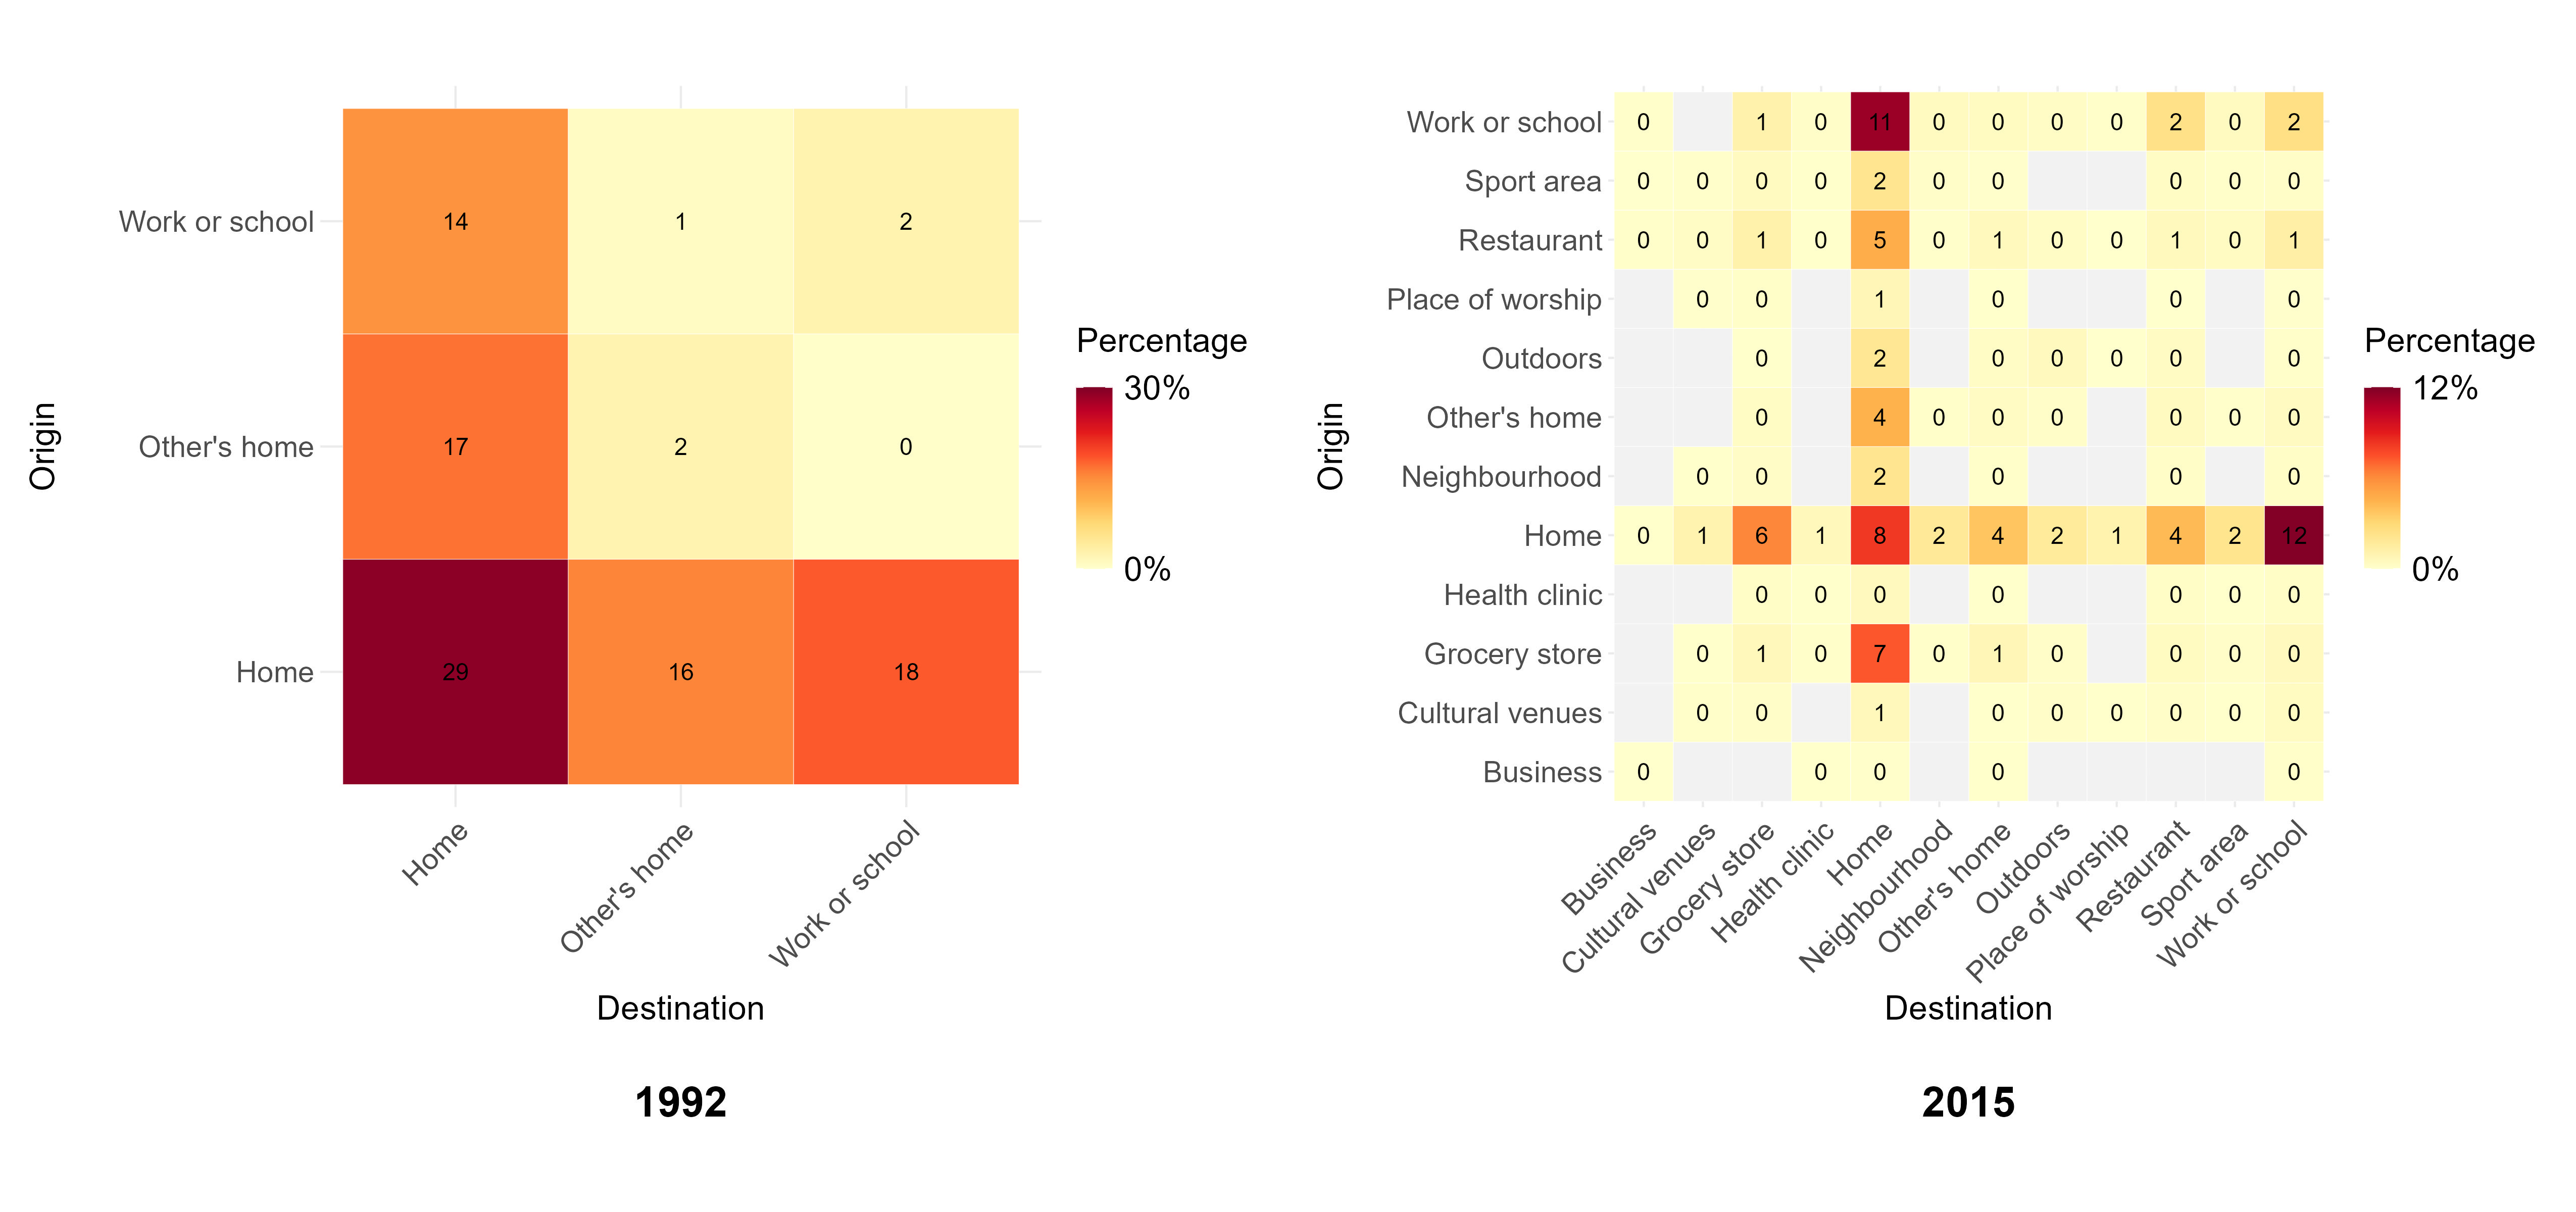
\includegraphics[width=1\linewidth]{Manuscript-figures/walking_hm_fig} 

}

\caption{Percentage of walking trips categorized by origin and destination}\label{fig:figure-01}
\end{figure}

For cycling trips, Figure \ref{fig:figure-02}, shows that in 1992, when
this mode of transportation was first included as an activity, the
majority of trips were from \texttt{home} to \texttt{work\ or\ school},
accounting for about 25\% of cases. This pattern remained in 2015, with
these trips representing 30\% of the cases. However, a notable change
occurred in \texttt{home} to \texttt{home} trips, which decreased
significantly from 19\% in 1992 to 5\% in 2015.

\begin{figure}

{\centering 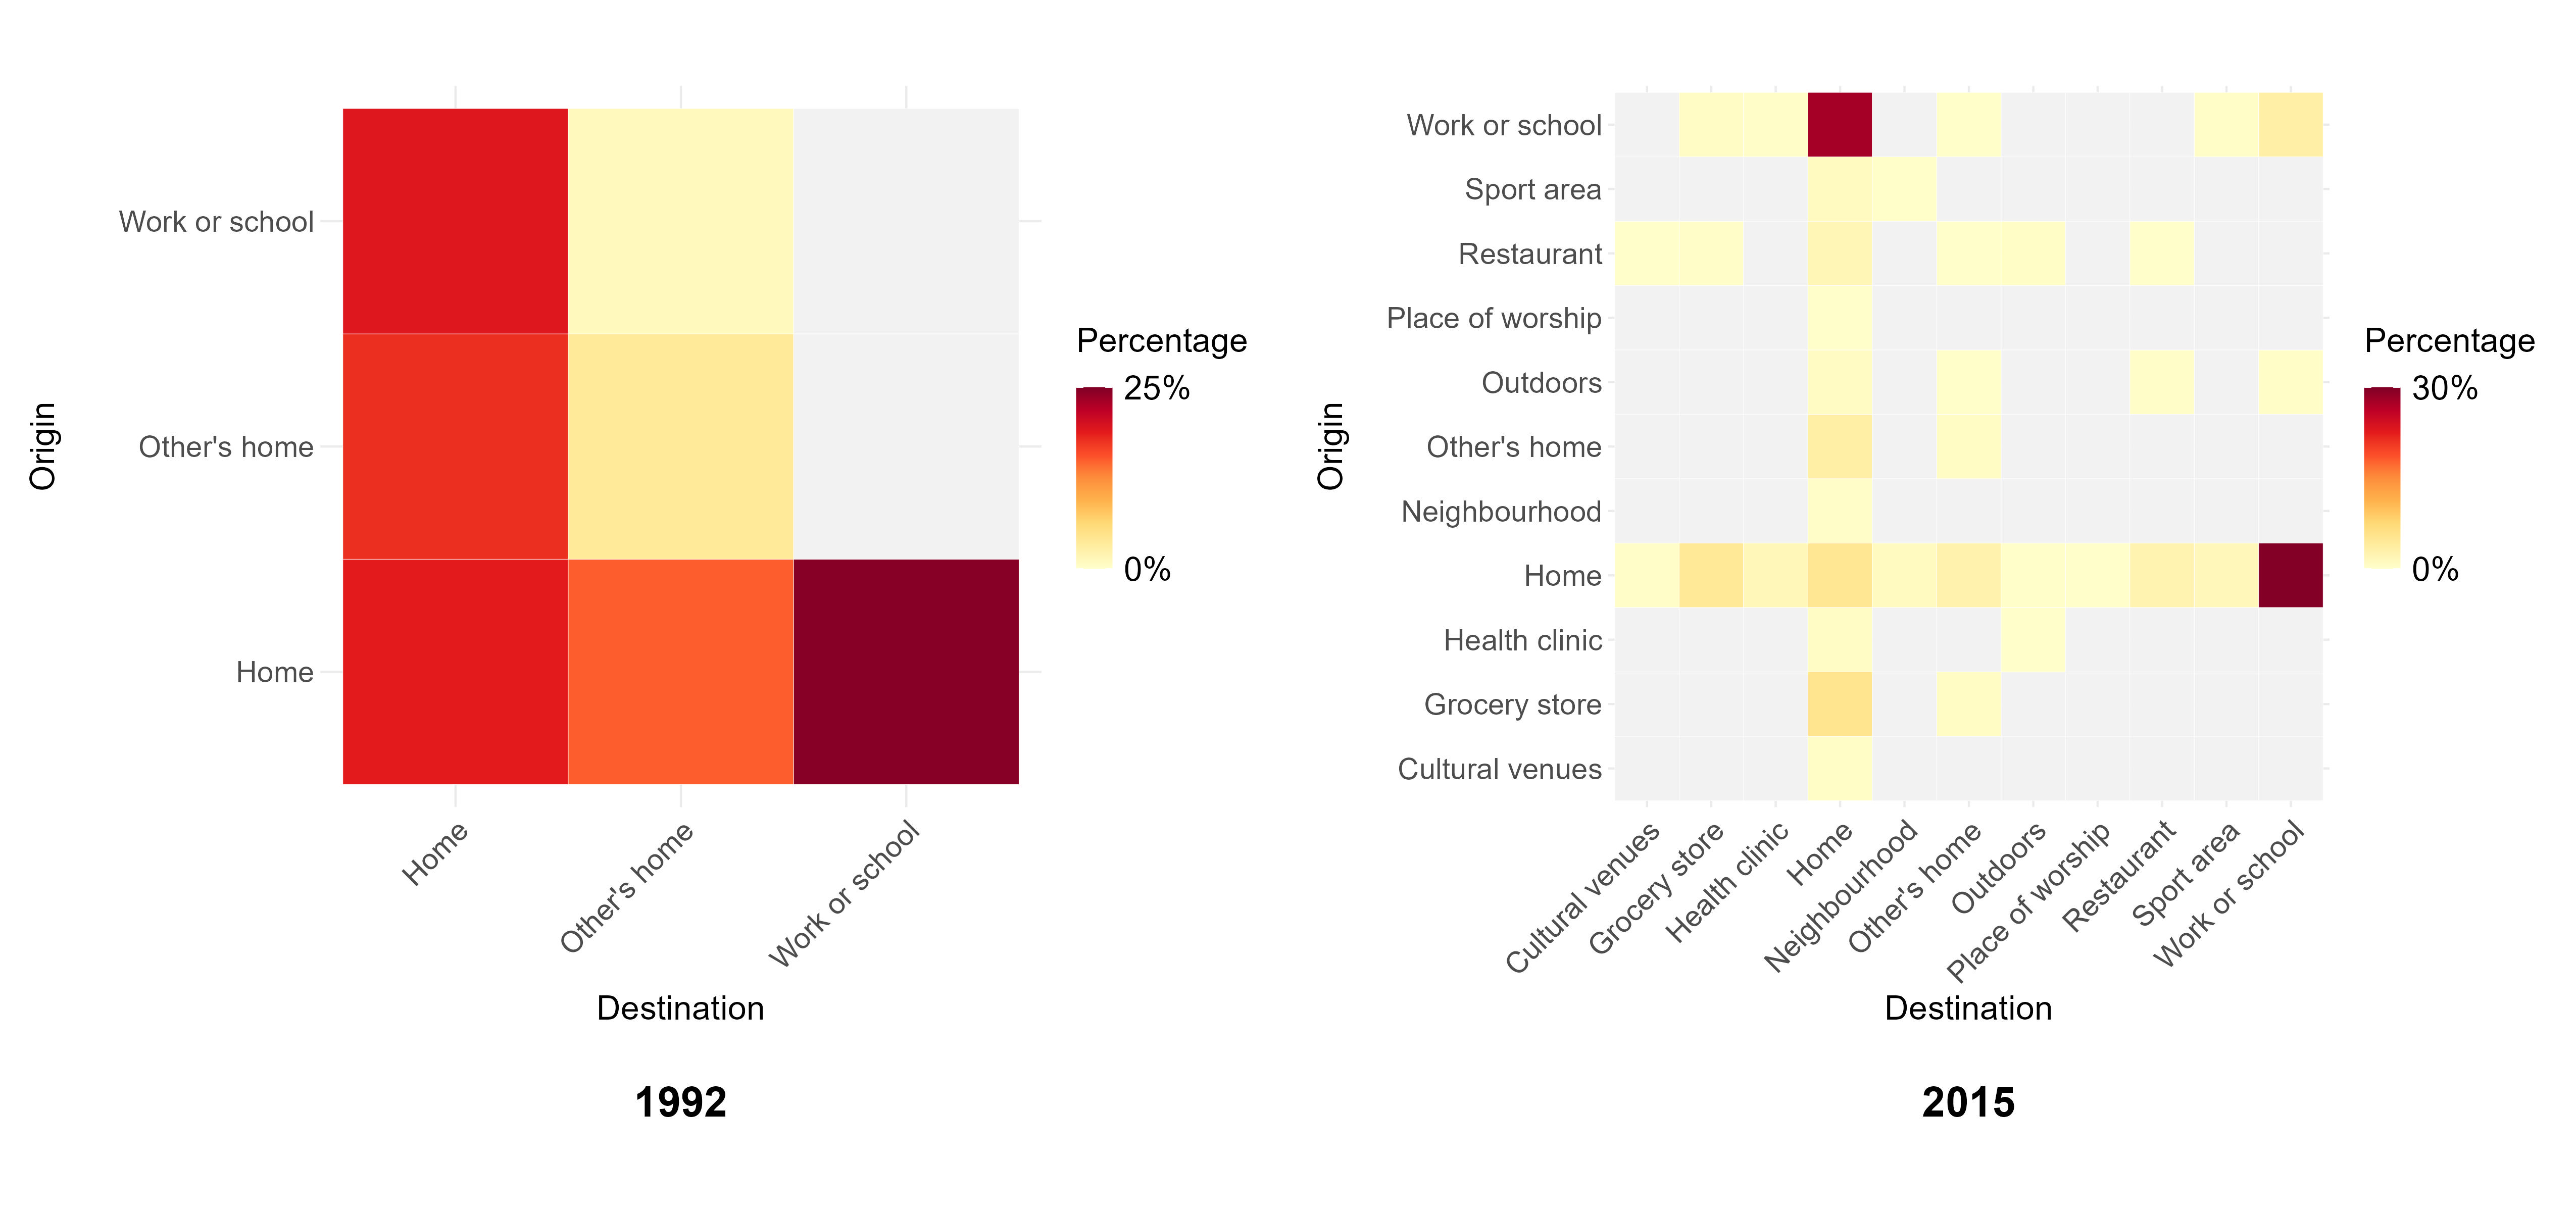
\includegraphics[width=1\linewidth]{Manuscript-figures/cycling_hm_fig} 

}

\caption{Percentage of cycling trips categorized by origin and destination}\label{fig:figure-02}
\end{figure}

\section{Python integration}\label{python-integration}

CAN WE PROVIDE PYTHON INTEGRATION? See here:

\url{https://github.com/paezha/idealista18/tree/master/Python}

\section{Concluding remarks}\label{concluding-remarks}

This paper presents \texttt{ActiveCA}, an open data product that
provides analysis-ready data from Cycles 2 (1986), 7 (1992), 12 (1998),
19 (2005), 24 (2010), and 29 (2015) of the GSS surveys on active travel
in Canada. In the form of an \texttt{R} data package, \{ActiveCA\} was
developed after collecting, cleaning, and processing the survey data,
providing information on origins, destinations, and duration of active
travel, as well other information.

It is important to remark that the present version of \{ActiveCA\}
covers all Canadian time use surveys up to 2015. While the most recent
time use survey was carried out in 2022 \citep{wray2024}, the Public Use
Microdata Files are currently unavailable, and at the moment it is
estimated that they will only be published in the later part of 2025.
The \texttt{R} package will be updated once these files become
available.

The value of \{ActiveCA\} lies in its transparency, accessibility, and
ease of use, which facilitates the addition of complementary data sets
in the future. \texttt{R} users can seamlessly explore GSS walking and
cycling episodes , with the option to suggest enhancements to the
package as needed. This article adopts the structure proposed by
Anastasia and Páez \citeyearpar{soukhov2023}, whose work provided
essential guidance for the creation of this package. Similarly, we aim
to contribute to the academic community by promoting transparent
research practices that encourage replication and innovation in related
fields. We believe that \{ActiveCA\} will serve as a basis for further
research on GSS and for the integration of additional data by the
authors or the wider open source community.

\section{Declaration of Conflicting
Interests}\label{declaration-of-conflicting-interests}

The author(s) declared no potential conflicts of interest with respect
to the research, authorship, and/or publication of this article.

\section{Funding}\label{funding}

The author(s) disclosed receipt of the following financial support for
the research, authorship, and/or publication of this article: This work
was supported by the Social Sciences and Humanities Research Council of
Canada (\emph{More description about the funding source after the review
process}).

\section{ORCID}\label{orcid}

Author 1

Author 2

Author 3

\section{Data availability statement}\label{data-availability-statement}

The \{ActiveCA\} R data package can be found and installed on Github
(\emph{link}).

\bibliographystyle{sageh}
\bibliography{bibfile.bib}


\end{document}
